\subsection{Specifications and Requirements}
This project idea requires the integration of power, systems, computer, optical, and web engineering to achieve a final product of a self-sustaining plant bed. The design in \autoref{fig:overall-block} shows four different subsystems the team has designated as power, control, sensing, and web.

\paragraph{Control}
The control subsystem is the brains of the entire operation. This subsystem has to accomplish four distinct tasks:
\begin{enumerate}
    \item Actuate mechanical components (linear rail, solenoid valve)
    \item Convert analog sensor data to digital data
    \item Send plant bed telemetry to web subsystem
    \item Receive commands from web subsystem and modify system accordingly
\end{enumerate}
In order to accomplish the first task, the chosen microcontroller (MCU) must be capable of driving the currents for these components and also support pulse-width modulation (PWM) for interacting with the motor controller. The second task requires that the MCU have an analog-to-digital converter. The third and fourth tasks necessitate WiFi connectivity as well as firmware support for either HTTP requests or WebSockets. These requirements for the control subsystem weigh heavily in the discussion of which MCU to choose found in Section \ref{sec:ps-control}.
\paragraph{Power}
The power system's function is self-explanatory, supply power to the entire system. This will be accomplished in two ways. First, using a DC barrel-plug to the wall, the system could be powered this way. The second way, is via the solar panels, batteries, and charge controller. Both manners of supplying power to the system must be regulated. Discussed in Section \ref{sec:ps-power} are the different ways that the charge controller can efficiently switch between battery power and the panels to increase battery health and charge level.
\paragraph{Sensing}
\paragraph{Web}
The web component of this project accomplishes three things; data analysis, reporting, and user specified control of components. The data analysis is occurring on the web because of the greater availability of compute power and greater ease of programmability. For reporting, the web will use databases to store data ad infinitum and serve this data in the form of graphs or ``live'' metrics. The web component also will be able to take a user's input to send commands back to the control system to actuate different parts such as the solenoids or to ask for a more recent data reading.
\subsubsection{Engineering Specifications}
\autoref{table:eng-specs} lays out the various metrics used to develop and design our project. 
\begin{table}[H]
    \caption{Engineering Specifications}
    \centering
    \begin{tabular}{c|c|c}
        \hline
        \textbf{Subsystem} & \textbf{Metric} & \textbf{Specification} \\\cline{2-3}
        \hline
        \multirow{19}{*}{\textbf{Control}} & Input voltage & 2.8-5.5 V \\ \cline{2-3}
                                        & Power consumption & $\leq$1.50W nominal power draw \\ \cline{2-3}
                                        & Shutdown power draw   & $\leq$10 uA \\ \cline{2-3}
                                        & Programmed in         & C++ or C \\ \cline{2-3}
                                        & Processor speed       & $\geq$20 MHz \\ \cline{2-3}
                                        & Processor cores       & $\geq$1 \\ \cline{2-3}
                                        & Memory                & $\geq$128 KB \\ \cline{2-3}
                                        & ADC resolution        & $\geq$8-bit \\ \cline{2-3}
                                        & ADC sampling rate     & $\geq$1 ksps \\ \cline{2-3}
                                        & ADC channels          & $\geq$4 channels \\ \cline{2-3}
                                        & Debug interface       & Yes \\ \cline{2-3}
                                        & Serial                & UART or I2C \\ \cline{2-3}
                                        & Transmit power        & $\geq$10 dBm \\ \cline{2-3}
                                        & Receive sensitivity   & $\geq$-50 dBm \\ \cline{2-3}
                                        & GPIO                  & $\geq$10 I/O \\ \cline{2-3}
                                        & Wireless connectivity & 802.11 (b or better) \\ \cline{2-3}
                                        & Internet protocol     & IPv4 \\ \cline{2-3}
                                        & Throughput            & $\geq$0.5 Mbps \\ \cline{2-3}
                                        & Network protocols     & TCP \\ \cline{2-3}
        \hline
        \multirow{2}{*}{\textbf{Power}} & Battery Life & 36 Hours \\
        \cline{2-3}
        & Some other metric & some other unit \\\cline{2-3}
        \hline
        \multirow{2}{*}{\textbf{Sensing}} & Spectra & 400nm - 1700nm \\
        \cline{2-3}
        & Resolution & \textless10nm \\\cline{2-3}
        \hline
        \multirow{2}{*}{\textbf{Web}} & Up-time & 95\textpm.1\% \\\cline{2-3}
                                    & Storage Capacity & \textgreater16 GB \\\cline{2-3}
                                    & Communication Methods & HTTP and WebSockets \\\cline{2-3}
        \hline
        \multirow{2}{*}{\textbf{Miscellaneous}} & Dimensions & 1 m\textsuperscript{3} \\
        \cline{2-3}
        & Weight\tablefootnote{The weight of the system includes a full soil load} & \textless 50lb \\
        \hline
    \end{tabular}
    \label{table:eng-specs}
\end{table}
\subsubsection{Marketing Requirements}
Find our House of Quality figure below:
\begin{figure}[H]
    \centering
    \caption{House of Quality}
    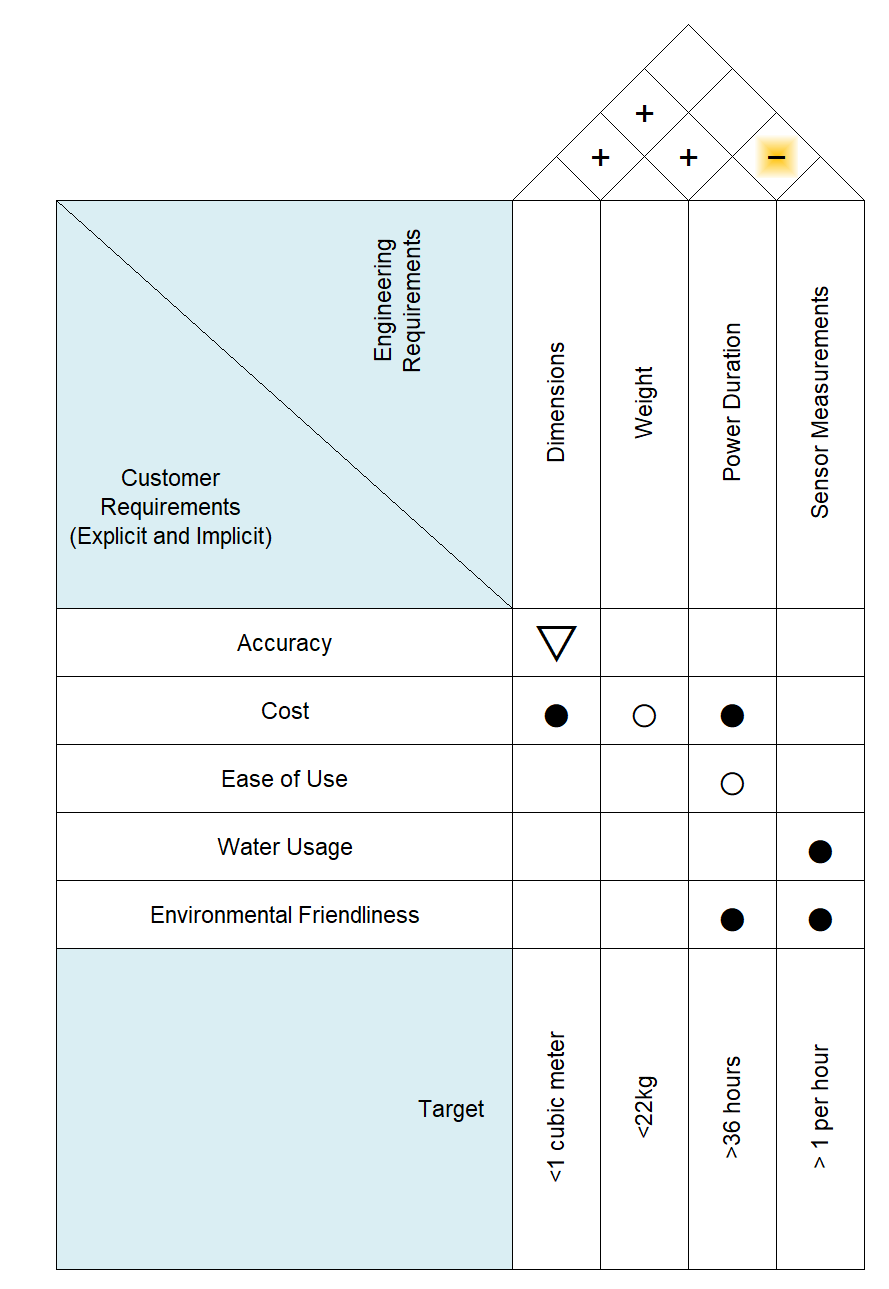
\includegraphics[width=.45\textwidth]{images/HouseOfQuality.PNG}
    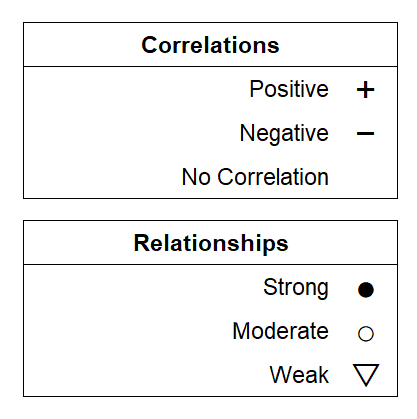
\includegraphics[width=.25\textwidth]{images/HouseOfQualityLegend.png}
\end{figure}
\begin{figure}[H]
    \caption{Overall block diagram}
    \centering
    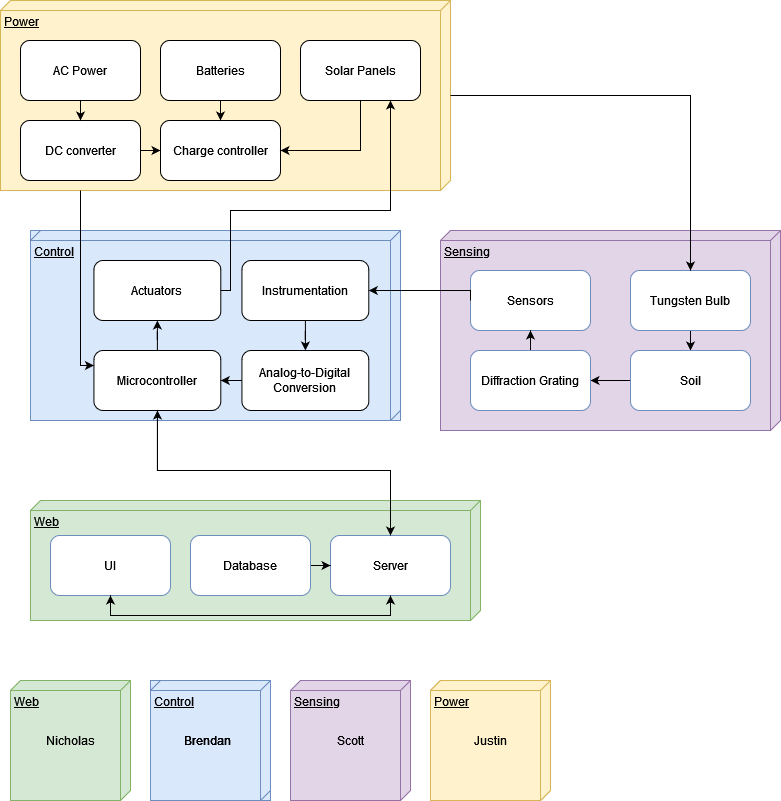
\includegraphics[width=\textwidth]{images/Overall Block Diagram.png}
    \label{fig:overall-block}
\end{figure}